\chapter{Appendix to chapter \ref{cha:mobilome}}

\section{Supplementary Figures}

\begin{figure}[h]
\centering
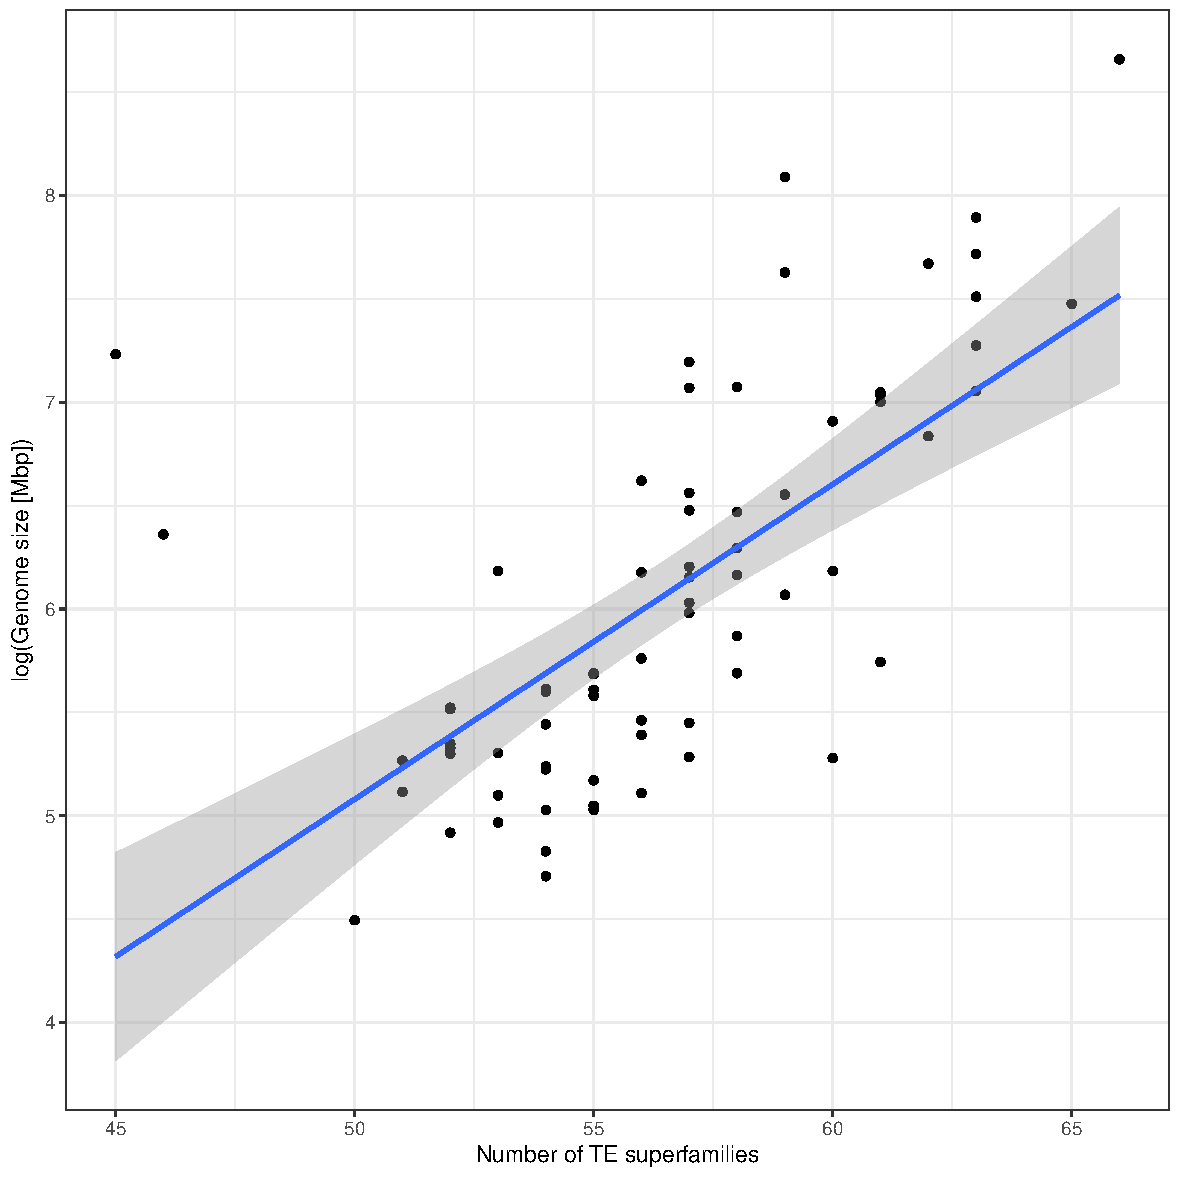
\includegraphics[width=0.7\textwidth]{te-families-vs-genome-size}
\caption[The number of TE superfamilies is significantly correlated to
genome size]{The number of TE superfamilies is significantly correlated to
genome size as well.}
\label{fig:te-families-vs-genome-size}
\end{figure}

\section{Supplementary Tables}

% Please add the following required packages to your document preamble:
% \usepackage{booktabs}
\begin{table}[]
\caption[TE coverage data]{{TE coverage by classes in 73 arthropod
genomes.%
\label{tab:coverage}}}
\begin{tabular}{@{}lllllllll@{}}
\toprule
Species                    & Genome size & DNA       & LINE      & LTR       & SINE      & Unknown    & Total      & Coverage {[}\%{]} \\ \midrule
Acromyrmex echinatior      & 295944863   & 14028877  & 5564391   & 3332023   & 321166    & 56838168   & 80084625   & 27.0606572414132  \\
Acyrthosiphon pisum        & 541675471   & 46850908  & 7139839   & 2352412   & 38433072  & 44085709   & 138861940  & 25.6356337760031  \\
Aedes aegypti              & 1383971543  & 284584199 & 170617062 & 74484211  & 19268167  & 224707931  & 773661570  & 55.9015518717208  \\
Agrilus planipennis        & 353849136   & 11965854  & 20658335  & 7721017   & 805978    & 45704697   & 86855881   & 24.5460203695396  \\
Anopheles gambiae          & 265011681   & 14556836  & 8430174   & 6904028   & 2383954   & 13962246   & 46237238   & 17.4472452782185  \\
Anoplophora glabripennis   & 707712193   & 80890038  & 14708125  & 3927741   & 65766     & 193744915  & 293336585  & 41.4485701816925  \\
Apis mellifera             & 250270657   & 1477978   & 93806     & 661247    & 0         & 8415504    & 10648535   & 4.25480762612934  \\
Athalia rosae              & 163837890   & 2189910   & 199632    & 415788    & 18659     & 4286428    & 7110417    & 4.33991001715171  \\
Atta cephalotes            & 317690795   & 14790388  & 3104389   & 1917120   & 80553     & 53276653   & 73169103   & 23.0315464443973  \\
Belgica antarctica         & 89583723    & 89347     & 225787    & 64091     & 0         & 1927767    & 2306992    & 2.57523568204461  \\
Blattella germanica        & 2055425512  & 118099518 & 96796661  & 3368694   & 41260001  & 566565387  & 826090261  & 40.1907175023913  \\
Bombus terrestris          & 248654244   & 3914003   & 2676528   & 1987158   & 9100      & 17941728   & 26528517   & 10.6688374078184  \\
Bombyx mori                & 481819406   & 14859808  & 52996846  & 2822023   & 45329577  & 66994932   & 183003186  & 37.9816968185794  \\
Camponotus floridanus      & 232685334   & 3588249   & 1189283   & 1820352   & 245858    & 19473445   & 26317187   & 11.310204449757   \\
Catajapyx silvestris       & 312272917   & 11564208  & 2999527   & 4563615   & 1450868   & 67274723   & 87852941   & 28.1333846828606  \\
Centruroides exilicauda    & 931068862   & 60232232  & 19922674  & 2827127   & 40425     & 129049264  & 212071722  & 22.7772327757214  \\
Ceratitis capitata         & 484773492   & 53984782  & 51057991  & 8093448   & 4481264   & 31292957   & 148910442  & 30.7175298273116  \\
Cimex lectularius          & 650492763   & 26133805  & 77196299  & 8906041   & 14201408  & 70965264   & 197402817  & 30.346658445453   \\
Copidosoma floridanum      & 645712421   & 24140234  & 15472247  & 28300530  & 1045178   & 77891713   & 146849902  & 22.7423071361361  \\
Culex quinquefasciatus     & 579042118   & 148830919 & 19232476  & 12525560  & 10422015  & 82116713   & 273127683  & 47.1688802091595  \\
Danaus plexippus           & 272853388   & 2556945   & 10476056  & 777496    & 1140231   & 13930574   & 28881302   & 10.5849160282371  \\
Daphnia pulex              & 197206209   & 3913500   & 1756846   & 11804780  & 1769569   & 20903178   & 40147873   & 20.3583209694985  \\
Drosophila ananassae       & 230993012   & 5851179   & 18214713  & 36010716  & 5878      & 32843785   & 92926271   & 40.2290399157183  \\
Drosophila erecta          & 152712140   & 1620381   & 7925820   & 12413050  & 5791      & 6927427    & 28892469   & 18.9195626490468  \\
Drosophila grimshawi       & 200467819   & 4081630   & 5726513   & 22750394  & 1989      & 7938263    & 40498789   & 20.202139775861   \\
Drosophila melanogaster    & 143726002   & 1864630   & 6201553   & 14975264  & 0         & 4411181    & 27452628   & 19.1006690633474  \\
Drosophila miranda         & 136728780   & 1193299   & 2169497   & 932607    & 12128     & 5964753    & 10272284   & 7.5128908485836   \\
Drosophila mojavensis      & 193826310   & 4423019   & 6200643   & 12547097  & 0         & 15174518   & 38345277   & 19.7833188899897  \\
Drosophila persimilis      & 188374079   & 3017923   & 10737250  & 21690609  & 44193     & 17715388   & 53205363   & 28.244524555844   \\
Drosophila pseudoobscura   & 152696384   & 1814141   & 4620512   & 9081564   & 6593      & 7604926    & 23127736   & 15.1462237638843  \\
Drosophila sechellia       & 166592095   & 4545125   & 10981352  & 16246960  & 0         & 5975207    & 37748644   & 22.6593248617229  \\
Drosophila simulans        & 124966452   & 454842    & 3082710   & 4363044   & 10511     & 1017167    & 8928274    & 7.14453667933215  \\
Drosophila virilis         & 206026697   & 2388960   & 7217526   & 14406968  & 2878      & 21536844   & 45553176   & 22.1103267990556  \\
Drosophila willistoni      & 235516348   & 6979192   & 13395864  & 30867252  & 12943     & 23060371   & 74315622   & 31.5543369413999  \\
Drosophila yakuba          & 165693946   & 2762860   & 7240428   & 18655858  & 4743      & 8220312    & 36884201   & 22.2604397386975  \\
Ephemera danica            & 475911277   & 1587870   & 4342127   & 657361    & 5788      & 103286144  & 109879290  & 23.0881879270955  \\
Euperipatoides rowelli     & 2681872052  & 81520224  & 68827726  & 43632247  & 1743681   & 591339224  & 787063102  & 29.3475261585671  \\
Eurytemora affinis         & 494890867   & 4913699   & 2873823   & 2975606   & 0         & 118249976  & 129013104  & 26.0690007843689  \\
Frankliniella occidentalis & 415803855   & 2366622   & 800197    & 769380    & 500775    & 36574762   & 41011736   & 9.86324092642191  \\
Gerris buenoi              & 1000194699  & 23294121  & 11729071  & 3527948   & 5436752   & 200880060  & 244867952  & 24.4820285735188  \\
Halyomorpha halys          & 1150099797  & 15071472  & 137983767 & 10173492  & 12033787  & 277888335  & 453150853  & 39.4010027809787  \\
Harpegnathos saltator      & 294465601   & 22402907  & 4860671   & 2536115   & 401040    & 38188633   & 68389366   & 23.2249083654427  \\
Heliconius melpomene       & 273786188   & 3309141   & 10787521  & 1806703   & 5675476   & 62279040   & 83857881   & 30.6289669367835  \\
Helicoverpa punctigera     & 432318525   & 1626618   & 8168605   & 684817    & 14403617  & 49299046   & 74182703   & 17.1592700081497  \\
Homalodisca vitripennis    & 2247672265  & 33258334  & 50290153  & 1400275   & 5082654   & 223402079  & 313433495  & 13.9448041371814  \\
Hyalella azteca            & 1181648033  & 17877377  & 22314001  & 1745793   & 6144      & 92142233   & 134085548  & 11.3473339146158  \\
Ixodes scapularis          & 1765382190  & 50926831  & 55077295  & 19711825  & 11668591  & 568841548  & 706226090  & 40.0041472039547  \\
Ladona fulva               & 1158111285  & 35625466  & 48467767  & 1277019   & 4772032   & 127344552  & 217486836  & 18.7794419082964  \\
Latrodectus hesperus       & 1137104758  & 64136256  & 27759711  & 8159512   & 8420167   & 79950721   & 188426367  & 16.570713091678   \\
Leptinotarsa decemlineata  & 1176182208  & 82875924  & 133162799 & 8299074   & 1354549   & 138863056  & 364555402  & 30.9948067162057  \\
Limnephilus lunatus        & 1333324643  & 27934987  & 62350860  & 529611    & 28296255  & 293532450  & 412644163  & 30.9485139396767  \\
Limulus polyphemus         & 1828256766  & 57602361  & 65031258  & 72495679  & 42695658  & 370231034  & 608055990  & 33.2587851612523  \\
Linepithema humile         & 219500750   & 3146879   & 1635451   & 1634508   & 124443    & 16888693   & 23429974   & 10.6742113637425  \\
Locusta migratoria         & 5759798599  & 548656473 & 922471727 & 110839523 & 122578589 & 1955778475 & 3660324787 & 63.5495273677711  \\
Loxosceles reclusa         & 3262503565  & 277060302 & 237214458 & 41355923  & 45464181  & 479023789  & 1080118653 & 33.1070489726806  \\
Lucilia cuprina            & 470583961   & 6587453   & 19759307  & 7925151   & 2180      & 85424374   & 119698465  & 25.4361548459149  \\
Machilis hrabei            & 2144866089  & 88401084  & 56089285  & 7823768   & 31164907  & 429393676  & 612872720  & 28.5739386315599  \\
Mayetiola destructor       & 185827756   & 2334815   & 634675    & 1332276   & 23062     & 14823623   & 19148451   & 10.3044084544615  \\
Mengenilla moldrzyki       & 155727465   & 11658097  & 2671635   & 5169197   & 18013     & 55690413   & 75207355   & 48.2942138690821  \\
Musca domestica            & 750403944   & 153293508 & 14279601  & 10470028  & 131797    & 218138285  & 396313219  & 52.8133177029251  \\
Nasonia vitripennis        & 295780872   & 9357282   & 9442807   & 12159327  & 93355     & 25283154   & 56335925   & 19.0465071723773  \\
Oncopeltus fasciatus       & 1098693218  & 24473805  & 59736772  & 6583561   & 17420216  & 123890779  & 232105133  & 21.1255634600632  \\
Onthophagus taurus         & 270546467   & 20788548  & 19283682  & 2900456   & 35890     & 51627557   & 94636133   & 34.9796225577767  \\
Orussus abietinus          & 201220334   & 2757902   & 424153    & 1413563   & 38403     & 34929859   & 39563880   & 19.6619691526802  \\
Pachypsylla venusta        & 701795784   & 18682836  & 13497373  & 754417    & 9711493   & 129459210  & 172105329  & 24.5235626835855  \\
Parasteatoda tepidariorum  & 1443909906  & 71202706  & 13909498  & 2196300   & 34445396  & 332296216  & 454050116  & 31.4458758204544  \\
Pediculus humanus          & 110781312   & 2419628   & 1040406   & 939937    & 226962    & 2807314    & 7434247    & 6.71074106795197  \\
Pogonomyrmex barbatus      & 235645958   & 6927372   & 1525631   & 3764006   & 113867    & 18340243   & 30671119   & 13.0157628250089  \\
Solenopsis invicta         & 396009169   & 15467507  & 7574738   & 8638636   & 0         & 82023961   & 113704842  & 28.7126791248614  \\
Strigamia maritima         & 176210797   & 2555637   & 1485499   & 20620465  & 342139    & 48848531   & 73852271   & 41.9113199970374  \\
Tribolium castaneum        & 210248733   & 8676449   & 1786295   & 624856    & 32802     & 32662849   & 43783251   & 20.8245017105525  \\
Trichogramma pretiosum     & 196221301   & 1988709   & 1912973   & 1512183   & 72212     & 19378013   & 24864090   & 12.671453034551   \\
Zootermopsis nevadensis    & 485009472   & 14695064  & 26646385  & 236056    & 9305656   & 70248697   & 121131858  & 24.9751530625777  \\ \bottomrule
\end{tabular}
\end{table}

% Please add the following required packages to your document preamble:
% \usepackage{booktabs}
\begin{table}[]
\caption[Genome assembly download URLs]{{Download URLs for the genome
assemblies of 73 arthropod species.%
\label{tab:urls}}}
\begin{tabular}{@{}lll@{}}
\toprule
Species                     & Order         & URL                                                                                                                                              \\ \midrule
Aedes aegypti                 & Diptera       & ftp://ftp.ncbi.nlm.nih.gov/genomes/all/GCA\_000004015.1\_Aedes\_aegypti/GCA\_000004015.1\_Aedes\_aegypti\_genomic.fna.gz                         \\
Atta cephalotes               & Hymenoptera   & ftp://ftp.ncbi.nlm.nih.gov/genomes/all/GCA\_000143395.2\_Attacep1.0/GCA\_000143395.2\_Attacep1.0\_genomic.fna.gz                                 \\
Acromyrmex echinatior         & Hymenoptera   & ftp://ftp.ncbi.nlm.nih.gov/genomes/all/GCA\_000204515.1\_Aech\_3.9/GCA\_000204515.1\_Aech\_3.9\_genomic.fna.gz                                   \\
Anopheles gambiae             & Diptera       & ftp://ftp.ncbi.nlm.nih.gov/genomes/all/GCA\_000005575.1\_AgamP3/GCA\_000005575.1\_AgamP3\_genomic.fna.gz                                         \\
Apis mellifera                & Hymenoptera   & ftp://ftp.ncbi.nlm.nih.gov/genomes/all/GCA\_000002195.1\_Amel\_4.5/GCA\_000002195.1\_Amel\_4.5\_genomic.fna.gz                                   \\
Acyrthosiphon pisum           & Hemiptera     & ftp://ftp.ncbi.nlm.nih.gov/genomes/all/GCA\_000142985.2\_Acyr\_2.0/GCA\_000142985.2\_Acyr\_2.0\_genomic.fna.gz                                   \\
Belgica antarctica            & Diptera       & ftp://ftp.ncbi.nlm.nih.gov/genomes/all/GCA\_000775305.1\_ASM77530v1/GCA\_000775305.1\_ASM77530v1\_genomic.fna.gz                                 \\
Bombyx mori                   & Lepidoptera   & ftp://ftp.ncbi.nlm.nih.gov/genomes/all/GCF\_000151625.1\_ASM15162v1/GCF\_000151625.1\_ASM15162v1\_genomic.fna.gz                                 \\
Bombus terrestris             & Hymenoptera   & ftp://ftp.ncbi.nlm.nih.gov/genomes/all/GCA\_000214255.1\_Bter\_1.0/GCA\_000214255.1\_Bter\_1.0\_genomic.fna.gz                                   \\
Camponotus floridanus         & Hymenoptera   & ftp://ftp.ncbi.nlm.nih.gov/genomes/all/GCA\_000147175.1\_CamFlo\_1.0/GCA\_000147175.1\_CamFlo\_1.0\_genomic.fna.gz                               \\
Culex quinquefasciatus        & Diptera       & ftp://ftp.ncbi.nlm.nih.gov/genomes/all/GCA\_000209185.1\_CulPip1.0/GCA\_000209185.1\_CulPip1.0\_genomic.fna.gz                                   \\
Drosophila ananassae          & Diptera       & ftp://ftp.ncbi.nlm.nih.gov/genomes/all/GCF\_000005115.1\_dana\_caf1/GCF\_000005115.1\_dana\_caf1\_genomic.fna.gz                                 \\
Drosophila erecta             & Diptera       & ftp://ftp.ncbi.nlm.nih.gov/genomes/all/GCF\_000005135.1\_dere\_caf1/GCF\_000005135.1\_dere\_caf1\_genomic.fna.gz                                 \\
Drosophila grimshawi          & Diptera       & ftp://ftp.ncbi.nlm.nih.gov/genomes/all/GCF\_000005155.2\_dgri\_caf1/GCF\_000005155.2\_dgri\_caf1\_genomic.fna.gz                                 \\
Drosophila melanogaster       & Diptera       & ftp://ftp.ncbi.nlm.nih.gov/genomes/all/GCA\_000001215.4\_Release\_6\_plus\_ISO1\_MT/GCA\_000001215.4\_Release\_6\_plus\_ISO1\_MT\_genomic.fna.gz \\
Drosophila miranda            & Diptera       & ftp://ftp.ncbi.nlm.nih.gov/genomes/all/GCA\_000269505.2\_DroMir\_2.2/GCA\_000269505.2\_DroMir\_2.2\_genomic.fna.gz                               \\
Drosophila mojavensis         & Diptera       & ftp://ftp.ncbi.nlm.nih.gov/genomes/all/GCF\_000005175.2\_dmoj\_caf1/GCF\_000005175.2\_dmoj\_caf1\_genomic.fna.gz                                 \\
Drosophila persimilis         & Diptera       & ftp://ftp.ncbi.nlm.nih.gov/genomes/all/GCF\_000005195.2\_dper\_caf1/GCF\_000005195.2\_dper\_caf1\_genomic.fna.gz                                 \\
Danaus plexippus              & Lepidoptera   & ftp://ftp.ncbi.nlm.nih.gov/genomes/all/GCA\_000235995.1\_DanPle\_1.0/GCA\_000235995.1\_DanPle\_1.0\_genomic.fna.gz                               \\
Drosophila pseudoobscura      & Diptera       & ftp://ftp.ncbi.nlm.nih.gov/genomes/all/GCF\_000001765.3\_Dpse\_3.0/GCF\_000001765.3\_Dpse\_3.0\_genomic.fna.gz                                   \\
Daphnia pulex                 & Cladocera     & ftp://ftp.ncbi.nlm.nih.gov/genomes/all/GCA\_000187875.1\_V1.0/GCA\_000187875.1\_V1.0\_genomic.fna.gz                                             \\
Drosophila sechellia          & Diptera       & ftp://ftp.ncbi.nlm.nih.gov/genomes/all/GCF\_000005215.3\_dsec\_caf1/GCF\_000005215.3\_dsec\_caf1\_genomic.fna.gz                                 \\
Drosophila simulans           & Diptera       & ftp://ftp.ncbi.nlm.nih.gov/genomes/all/GCA\_000754195.2\_ASM75419v2/GCA\_000754195.2\_ASM75419v2\_genomic.fna.gz                                 \\
Drosophila virilis            & Diptera       & ftp://ftp.ncbi.nlm.nih.gov/genomes/all/GCF\_000005245.1\_dvir\_caf1/GCF\_000005245.1\_dvir\_caf1\_genomic.fna.gz                                 \\
Drosophila willistoni         & Diptera       & ftp://ftp.ncbi.nlm.nih.gov/genomes/all/GCF\_000005925.1\_dwil\_caf1/GCF\_000005925.1\_dwil\_caf1\_genomic.fna.gz                                 \\
Drosophila yakuba             & Diptera       & ftp://ftp.ncbi.nlm.nih.gov/genomes/all/GCA\_000005975.1\_dyak\_caf1/GCA\_000005975.1\_dyak\_caf1\_genomic.fna.gz                                 \\
Heliconius melpomene          & Lepidoptera   & ftp://ftp.ncbi.nlm.nih.gov/genomes/all/GCA\_000313835.2\_ASM31383v2/GCA\_000313835.2\_ASM31383v2\_genomic.fna.gz                                 \\
Harpegnathos saltator         & Hymenoptera   & ftp://ftp.ncbi.nlm.nih.gov/genomes/all/GCA\_000147195.1\_HarSal\_1.0/GCA\_000147195.1\_HarSal\_1.0\_genomic.fna.gz                               \\
Ixodes scapularis             & Ixodida       & ftp://ftp.ncbi.nlm.nih.gov/genomes/all/GCA\_000208615.1\_JCVI\_ISG\_i3\_1.0/GCA\_000208615.1\_JCVI\_ISG\_i3\_1.0\_genomic.fna.gz                 \\
Linepithema humile            & Hymenoptera   & ftp://ftp.ncbi.nlm.nih.gov/genomes/all/GCA\_000217595.1\_Lhum\_UMD\_V04/GCA\_000217595.1\_Lhum\_UMD\_V04\_genomic.fna.gz                         \\
Locusta migratoria            & Orthoptera    & ftp://ftp.ncbi.nlm.nih.gov/genomes/all/GCA\_000516895.1\_LocustGenomeV1/GCA\_000516895.1\_LocustGenomeV1\_genomic.fna.gz                         \\
Limulus polyphemus            & Xiphosura     & ftp://ftp.ncbi.nlm.nih.gov/genomes/all/GCA\_000517525.1\_Limulus\_polyphemus-2.1.2/GCA\_000517525.1\_Limulus\_polyphemus-2.1.2\_genomic.fna.gz   \\
Mayetiola destructor          & Diptera       & ftp://ftp.ncbi.nlm.nih.gov/genomes/all/GCA\_000149185.1\_Mdes\_1.0/GCA\_000149185.1\_Mdes\_1.0\_genomic.fna.gz                                   \\
Musca domestica               & Diptera       & ftp://ftp.ncbi.nlm.nih.gov/genomes/all/GCF\_000371365.1\_Musca\_domestica-2.0.2/GCF\_000371365.1\_Musca\_domestica-2.0.2\_genomic.fna.gz         \\
Mengenilla moldrzyki          & Strepsiptera  & ftp://ftp.ncbi.nlm.nih.gov/genomes/all/GCA\_000281935.1\_Memo\_1.0/GCA\_000281935.1\_Memo\_1.0\_genomic.fna.gz                                   \\
Nasonia vitripennis           & Hymenoptera   & ftp://ftp.ncbi.nlm.nih.gov/genomes/all/GCA\_000002325.2\_Nvit\_2.1/GCA\_000002325.2\_Nvit\_2.1\_genomic.fna.gz                                   \\
Pogonomyrmex barbatus         & Hymenoptera   & ftp://ftp.ncbi.nlm.nih.gov/genomes/all/GCA\_000187915.1\_Pbar\_UMD\_V03/GCA\_000187915.1\_Pbar\_UMD\_V03\_genomic.fna.gz                         \\
Pediculus humanus             & Phthiraptera  & ftp://ftp.ncbi.nlm.nih.gov/genomes/all/GCA\_000006295.1\_JCVI\_LOUSE\_1.0/GCA\_000006295.1\_JCVI\_LOUSE\_1.0\_genomic.fna.gz                     \\
Solenopsis invicta            & Hymenoptera   & ftp://ftp.ncbi.nlm.nih.gov/genomes/all/GCA\_000188075.1\_Si\_gnG/GCA\_000188075.1\_Si\_gnG\_genomic.fna.gz                                       \\
Strigamia maritima            & Myriapoda     & ftp://ftp.ncbi.nlm.nih.gov/genomes/all/GCA\_000239455.1\_Smar\_1.0/GCA\_000239455.1\_Smar\_1.0\_genomic.fna.gz                                   \\
Tribolium castaneum           & Coleoptera    & ftp://ftp.ncbi.nlm.nih.gov/genomes/all/GCA\_000002335.2\_Tcas\_3.0/GCA\_000002335.2\_Tcas\_3.0\_genomic.fna.gz                                   \\
Zootermopsis nevadensis       & Isoptera      & ftp://ftp.ncbi.nlm.nih.gov/genomes/all/GCA\_000696155.1\_ZooNev1.0/GCA\_000696155.1\_ZooNev1.0\_genomic.fna.gz                                   \\
Agrilus planipennis Fairmaire & Coleoptera    & ftp://ftp.hgsc.bcm.edu/I5K-pilot/Emerald\_ash\_borer/NCBI-submitted/Aplan.agp.contamination-free.scaffolds.50.fa                                 \\
Anoplophora glabripennis      & Coleoptera    & ftp://ftp.hgsc.bcm.edu/I5K-pilot/Asian\_long-horned\_beetle/Agla\_Btl03082013.genome.fa                                                          \\
Athalia rosae                 & Hymenoptera   & ftp://ftp.hgsc.bcm.edu/I5K-pilot/Turnip\_sawfly/Aros01112013-genome.fa                                                                           \\
Blattella germanica           & Blattodea     & ftp://ftp.hgsc.bcm.edu/I5K-pilot/German\_cockroach/Bgermanica.scaffolds                                                                          \\
Catajapyx silvestris          & Diplura       & ftp://ftp.hgsc.bcm.edu/I5K-pilot/Silvestris\_Northern\_Forcepstail/forcepstail.consistent.scaffolds                                              \\
Centruroides exilicauda       & Scorpiones    & ftp://ftp.hgsc.bcm.edu/I5K-pilot/Bark\_scorpion/NCBI-submitted/Cscul.scaffolds.50.fa                                                             \\
Ceratitis capitata            & Diptera       & ftp://ftp.hgsc.bcm.edu/I5K-pilot/Mediterranean\_fruit\_fly/Ccap01172013-genome.fa                                                                \\
Cimex lectularius             & Hemiptera     & ftp://ftp.hgsc.bcm.edu/I5K-pilot/Bed\_bug/Clec\_Bbug02212013.genome.fa                                                                           \\
Copidosoma floridanum         & Hymenoptera   & ftp://ftp.hgsc.bcm.edu/I5K-pilot/Copidosoma\_floridanum/NCBI-submitted/Cflo.scaffolds.50.fa                                                      \\
Ephemera danica               & Ephemeroptera & ftp://ftp.hgsc.bcm.edu/I5K-pilot/Mayfly/Edan07162013.scaffolds.fa                                                                                \\
Euperipatoides rowelli        & Euonychophora & ftp://ftp.hgsc.bcm.edu/I5K-pilot/Velvet\_worm/pre\_assembly/Erow.scaffolds.fasta                                                                 \\
Eurytemora affinis            & Calanoida     & ftp://ftp.hgsc.bcm.edu/I5K-pilot/Eurytemora\_affinis/NCBI-submitted/Eaff\_11172013.genome.fa                                                     \\
Frankliniella occidentalis    & Thysanoptera  & ftp://ftp.hgsc.bcm.edu/I5K-pilot/Western\_flower\_thrips/NCBI-submitted/Focc.scaffolds                                                           \\
Gerris buenoi                 & Hemiptera     & ftp://ftp.hgsc.bcm.edu/I5K-pilot/Water\_strider/NCBI-submitted/Gbue\_1.0-unplaced\_scaffolds.fsa                                                 \\
Halyomorpha halys             & Hemiptera     & ftp://ftp.hgsc.bcm.edu/I5K-pilot/Brown\_marmorated\_stink\_bug/Hhal.scaffolds.fa                                                                 \\
Helicoverpa punctigera        & Lepidoptera   & ftp://ftp.hgsc.bcm.edu/I5K-pilot/Helicoverpa\_punctigera/Hpun12202012.genome.fa                                                                  \\
Homalodisca vitripennis       & Hemiptera     & ftp://ftp.hgsc.bcm.edu/I5K-pilot/Glassy-winged\_sharpshooter/NCBI-submitted/Hvit.scaffolds                                                       \\
Hyalella azteca               & Amphipoda     & ftp://ftp.hgsc.bcm.edu/I5K-pilot/Hyalella\_azteca/pre\_assembly/Hazt.scaffolds.fasta                                                             \\
Ladona fulva                  & Odonata       & ftp://ftp.hgsc.bcm.edu/I5K-pilot/Scarce\_Chaser/Lful\_Scha04012013-genome.fa                                                                     \\
Latrodectus hesperus          & Araneae       & ftp://ftp.hgsc.bcm.edu/I5K-pilot/Western\_black\_widow\_spider/NCBI-submitted/Lhes.scaffolds                                                     \\
Leptinotarsa decemlineata     & Coleoptera    & ftp://ftp.hgsc.bcm.edu/I5K-pilot/Colorado\_Potato\_Beetle/Ldec.genome.10062013.fa                                                                \\
Limnephilus lunatus           & Trichoptera   & ftp://ftp.hgsc.bcm.edu/I5K-pilot/Caddisfly/NCBI-submitted/Llun.contaminationfree.scaffolds.fa                                                    \\
Loxosceles reclusa            & Araneae       & ftp://ftp.hgsc.bcm.edu/I5K-pilot/Brown\_recluse\_spider/NCBI-submitted/Lrec.scaffolds                                                            \\
Lucilia cuprina               & Diptera       & ftp://ftp.hgsc.bcm.edu/I5K-pilot/Sheep\_blowfly/NCBIsubmitted/Lcup.scaffolds                                                                     \\
Machilis hrabei               & Archaeognatha & ftp://ftp.hgsc.bcm.edu/I5K-pilot/Hrabes\_jumping\_bristletail/pre-assembly/Mhar.scaffolds.fasta                                                  \\
Oncopeltus fasciatus          & Hemiptera     & ftp://ftp.hgsc.bcm.edu/I5K-pilot/Milkweed\_bug/NCBI-submitted/Ofas.contaminationfree.scaffolds                                                   \\
Onthophagus taurus            & Coleoptera    & ftp://ftp.hgsc.bcm.edu/I5K-pilot/Bull-headed\_Dung\_beetle/Otaur.scaffolds.fa                                                                    \\
Orussus abietinus             & Hymenoptera   & ftp://ftp.hgsc.bcm.edu/I5K-pilot/Parasitic\_wood\_wasp/Oabi11242013.genome.fa                                                                    \\
Pachypsylla venusta           & Hemiptera     & ftp://ftp.hgsc.bcm.edu/I5K-pilot/Hackberry\_petiole\_gall\_psyllid/NCBI-submitted/Pven.scaffolds.50.fa                                           \\
Parasteatoda tepidariorum     & Araneae       & ftp://ftp.hgsc.bcm.edu/I5K-pilot/Common\_house\_spider/NCBI-submitted/Ptep01282013.genome.fa                                                     \\
Trichogramma pretiosum        & Hymenoptera   & ftp://ftp.hgsc.bcm.edu/I5K-pilot/Trichogramma\_pretiosum/Tpre\_scaffolds.50.fa                                                                   \\ \bottomrule
\end{tabular}
\end{table}

% Please add the following required packages to your document preamble:
% \usepackage{booktabs}
\begin{table}[]
\caption[Word patterns to exclude non-TE search hits]{{Patterns employed to exclude non-TE search hits. Note
that these are regular expression for use with a compatible parser such
as GNU grep or Perl.\label{tab:patterns}}}
\centering
\begin{tabular}{@{}l@{}}
\toprule
Pattern               \\ \midrule
transcripta           \\
transpos              \\
gag{[}-/{]}pol        \\
env(elope)? protein   \\
env\textbackslash{}b  \\
pol p(olyp)?rotein    \\
gag(-like)? protein   \\
reverse transcrpitase \\
retro                 \\
integras              \\
replicas              \\
t-element             \\
transporase           \\
piggybac              \\
copia                 \\ \bottomrule
\end{tabular}
\end{table}
